\documentclass[12pt]{article}
\usepackage{amsmath}
\usepackage{graphicx}
\usepackage{hyperref}
\usepackage[utf8]{inputenc}
\usepackage{geometry}
\usepackage{mathtools}
\usepackage{empheq}
\usepackage{listings}
\usepackage{xcolor}
\usepackage{authblk}
\usepackage{subcaption}
\usepackage{svg}
\usepackage{minted}


\definecolor{LightGray}{gray}{0.9}

\graphicspath{ {./assets/} }
\geometry{margin=0.75in}

\title{HW}
\date{}

\begin{document}

\begin{enumerate}

    \item Problem 1
    
    \begin{align*}
        P &= \frac{2 \pi^2 k_B^4}{15 c^2 h^3} T^4 \\
        & \text{SA} = 0.65 \text{ m$^2$} \\
        & T = 34 \text{$^\circ$C} = 307.15 \text{ K} \\
        P &= \epsilon \sigma T^4 \\
        P &= 1 \cdot 5.670 \cdot 10^{-8} \text{ J/m$^2$/s/K$^4$} \cdot \left(307.15 \text{ K}\right)^4 \\
        P &= 504.6 \text{ J/m$^2$/s} \\
        P &= 504.6 \text{ J/m$^2$/s} \cdot 0.65 \text{ m$^2$} \\
        \Aboxed{P &= 328.02 \text{W}}
    \end{align*}

    \newpage
    \item Problem 2 (2.5)
    
    \begin{align*}
        \lambda_{\text{max}} &= \frac{hc}{5k_BT} \\
        h &= \frac{\lambda_{\text{max}}5k_BT}{c} \\
        \lambda_{\text{max}} &= \frac{c_2}{5T} \\
        & c_2 = 1.434 \cdot 10^{-2} \\
        & k_B = 1.38 \cdot 10^{-23} \text{ J/K} \\
        & c = 3 \cdot 10^{8} \text{ m/s}
    \end{align*}

    \begin{tabular}{|c|c|c|}
        \hline
        T (K) & $\lambda_{\text{max}}$ & $h = \frac{\lambda_{\text{max}}5k_BT}{c}$ \\
        \hline
        1646 & $1.75 \cdot 10^{-6}$ & $6.626 \cdot 10^{-34}$ J/s \\
        1449 & $2.1 \cdot 10^{-6}$ & $6.998 \cdot 10^{-34}$ J/s \\
        1259 & $2.3 \cdot 10^{-6}$ & $6.66 \cdot 10^{-34}$ J/s \\
        \hline
    \end{tabular}

    $\boxed{h_{\text{avg}} = 6.76 \cdot 10^{-34} \text{ J/s}}$

    \newpage
    \item Problem 3 (2.7)
    
    \begin{align*}
        <\nu> &= \frac{3N_ah\nu}{\exp\left(h\nu/\left(k_BT\right)\right)-1} \\
        \nu = \frac{c}{\lambda} \\
        & h = 6.626 \cdot 10^{-34} \\
        & c = 3 \cdot 10^{8} \\
        & k_B = 1.38 \cdot 10^{-23} \\
        & T = 1635 \text{ K} \\
        k_B \cdot T &= 2.258 \cdot 10^{-20}
    \end{align*}

    \begin{tabular}{|c|c|c|c|c|}
        \hline
        $\lambda$ ($\mu$m) & $\nu$ s$^{-1}$ & $h\nu$ & $\frac{h\nu}{k_BT}$ (J) & $<\nu> = \frac{3N_ah\nu}{\exp\left(h\nu/\left(k_BT\right)\right)-1}$ (J) \\
        \hline
        1 & $2.998\cdot10^{14}$ & $1.986\cdot10^{-19}$ & 8.797 & $3.002\cdot10^{-23}$ \\
        2 & $1.499\cdot10^{14}$ & $9.932\cdot10^{-20}$ & 4.399 & $1.236\cdot10^{-21}$ \\
        5 & $5.996\cdot10^{13}$ & $3.973\cdot10^{-20}$ & 1.759 & $8.261\cdot10^{-21}$ \\
        20 & $1.499\cdot10^{13}$ & $9.932\cdot10^{-19}$ & 0.440 & $1.798\cdot10^{-20}$ \\
        \hline
    \end{tabular}

    The wavelength of 1 $\mu$m has the smallest energy. Therefore, at this wavelength, most of the photons will have zero energy.

    \newpage
    \item Problem 4 (2.9)
    
    Average Vibrational energy

    S1 T = 400K $\nu = 12 \cdot 10^{12}$ s$^{-1}$

    a)

    \begin{align*}
        <\nu_{\text{vib}}> &= \frac{3N_ah\nu}{\exp\left(h\nu/\left(k_BT\right)\right)-1} \\
        <\nu_{\text{vib}}> &= \frac{3 \cdot 6.02 \cdot 10^{23} \cdot 6.626 \cdot 10^{-34} \cdot 12 \cdot 10^{-12}}{\exp\left[6.626 \cdot 10^{-34} \cdot 12 \cdot 10^{-12} / \left(1.38 \cdot 10^{-23} \cdot 400\right)\right]-1} \\
        \Aboxed{<\nu_{\text{vib}}> &= 4457 \text{ J/mol}}
    \end{align*}

    b)

    $\boxed{3N_ah\nu = 14364 \text{ J/mol}}$
    
    \newpage
    \item Problem 5 (2.11)
    
    \begin{align*}
        \lambda \nu &= c \\
        \nu &= \frac{c}{\lambda} \\
        & c = 3 \cdot 10^{8} \text{ m/s} \\
        & 1 \text{ eV} = 1.602 \cdot 10^{-19} \text{ J}
    \end{align*}

    Convert wavelength to frequency and kinetic energy from eV to J.

    Tabulated values:

    \begin{tabular}{|c|c|c|c|}
        \hline
        $\lambda$ (nm) & KE (eV) & $\nu$ (Hz) & KE (J) \\
        \hline
        261 & 0.13 & 1.15$\cdot 10^{15}$ & 2.08$\cdot 10^{-20}$ \\
        250 & 0.33 & 1.20$\cdot 10^{15}$ & 5.29$\cdot 10^{-20}$ \\ 
        234 & 0.68 & 1.28$\cdot 10^{15}$ & 1.09$\cdot 10^{-19}$ \\
        218	& 1.08 & 1.38$\cdot 10^{15}$ & 1.73$\cdot 10^{-19}$ \\ 
        184	& 2.13 & 1.63$\cdot 10^{15}$ & 3.41$\cdot 10^{-19}$ \\
        \hline
    \end{tabular}

    \[ E_k = h \nu - \phi \]

    Fitting the data to the above equation yields:

    \[ E_k = 6.68 \cdot 10^{-34} \cdot \nu - 7.48 \cdot 10^{-19} \]

    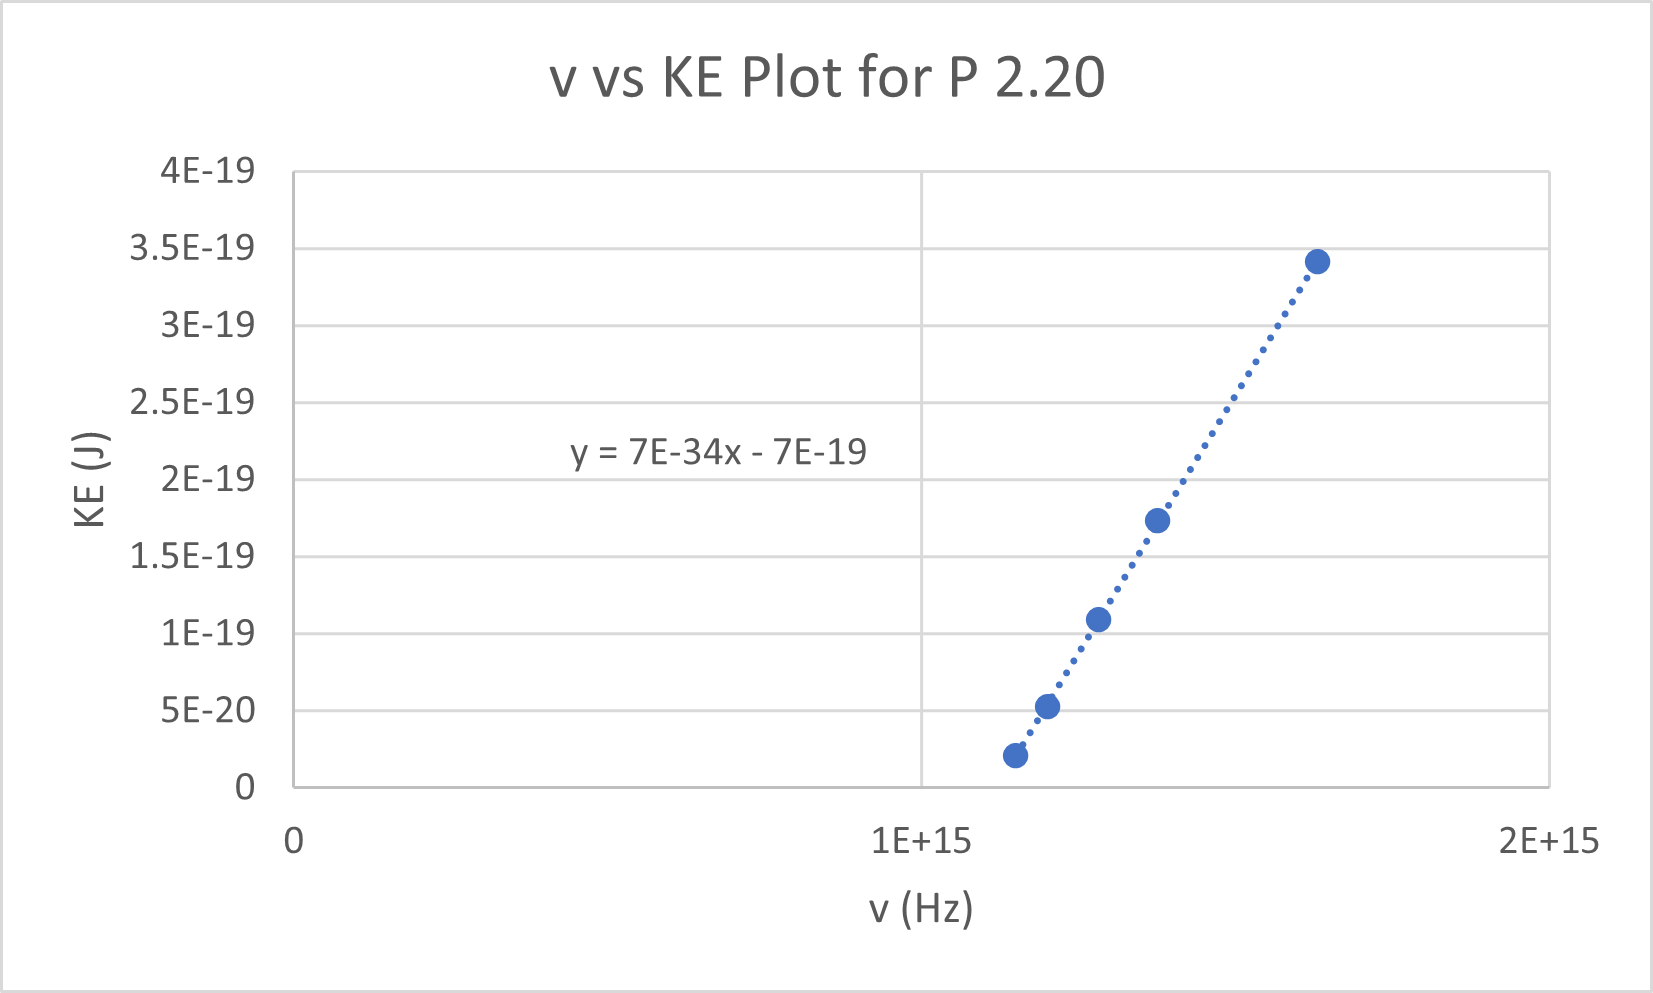
\includegraphics{assets/p6.png}

    $\boxed{h = 6.68 \cdot 10^{-34} \text{ J$\cdot$s}}$

    $\phi = 7.48 \cdot 10^{-19}$
    
    $\boxed{\phi = 4.67 \text{ eV}}$

    \newpage
    \item Problem 6 (2.20)
    
    a.
    
    \begin{align*}
        & \text{MW}_{\text{H}_2} = 2.016 \text{ g/mol} \\
        \text{m}_{\text{H}_2} &= \frac{2.016 \text{ g/mol}}{6.022 \cdot 10^{23} \text{ mol$^{-1}$}} \cdot \frac{1 \text{ kg}}{1000 \text{ g}} \\
        \text{m}_{\text{H}_2} &= 3.35 \cdot 10^{-27} \text{ kg} \\
        \intertext{Photon momentum}
        p &= \frac{h}{\lambda} \\
        \intertext{Particle momentum}
        p &= mv \\
        \intertext{Momentum is conserved}
        mv &= \frac{h}{\lambda} \\
        v &= \frac{h}{\lambda m} \\
        v &= \frac{6.62 \cdot 10^{-34} \text{ J$\cdot$s}}{5.84 \cdot 10^{-8} \text{m} \cdot 3.35 \cdot 10^{-27} \text{ kg}} \\
        \Aboxed{v &= 3.39 \text{ m/s}}
    \end{align*}

    b.

    \begin{align*}
        \text{KE} &= \frac{1}{2} m v^2 \\
        \text{KE} &= \frac{1}{2} \cdot 3.35 \cdot 10^{-27} \text{ kg} \cdot \left(3.39 \text{ m/s}\right)^2 \cdot 6.022 \cdot 10^{23} \text{ mol$^{-1}$} \\
        \Aboxed{\text{KE} &= 1.16 \cdot 10^{-2} \text{ J/mol}}
    \end{align*}

\end{enumerate}

\end{document}